\documentclass{article}
\usepackage[utf8]{inputenc}
\usepackage{amsfonts}
\usepackage{amsmath}
\usepackage{graphicx}
\usepackage[a4paper, total={6in, 8in}]{geometry}
\usepackage{setspace}
\usepackage{enumitem}
\usepackage{xparse}
\usepackage{tkz-tab}


\everymath{\displaystyle}

\newcommand\tab[1][1cm]{\hspace*{#1}}
\doublespacing
\author{Frederic Becerril}

\NewDocumentCommand{\mylim}{ O{n} O{\infty}}{\underset{#1 \rightarrow #2}{\longrightarrow}}
\newcommand{\mysim}[2]{\underset{#1 \rightarrow #2}{\sim}}
\newcommand{\mysupp}[1]{\underset{x \in #1}{Sup}}
% \newcommand{\citer}[2]{\og #2 \fg{} (#1)}

\begin{document}

\part*{Exerice 2}

$f_n(x) = \frac{x}{x + n}$\\
$\bullet$ Soit $x \in \mathbb{R}_+ \tab \frac{x}{x+n}\mylim 0$\\
Donc $f_n$ converge simplement vers la fonction $0$\\
$\bullet$ $f_n(x)' = \frac{x + n - x}{(x + n)^2} = \frac{n}{(x+n)^2}$\\
Or $n \geq 0$ et $(x + n)^2 \geq 0$ donc $f_n(x)' \geq 0$\\
$f_n(0) = \frac{0}{0 + n} = 0$\\
$f_n(x) \mylim[x][\infty] = 1$
\\

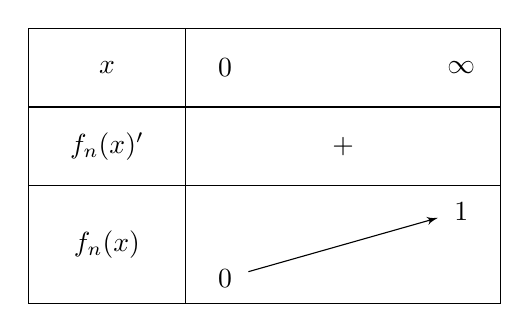
\begin{tikzpicture}
    \tkzTabInit{$x$ / 1 , $f_n(x)'$ / 1, $f_n(x)$ / 1.5}{$0$, $\infty$}
    \tkzTabLine{, +, }
    \tkzTabVar{-/ 0, +/ 1,}
\end{tikzpicture}\\
$||f_n(x) - f(x)||_{\infty} = \underset{x\in\mathbb{R}_+}{Sup} |f_n(x) - f(x)| = \mysupp{\mathbb{R_+}} f_n(x) = 1$\\
Donc $||f_n(x) - f(x)||_{\infty} \neq 0$ donc la suite $(f_n)$ ne converge pas uniformement vers 0\\
Soit $a \in \mathbb{R}$ on a que $\mysupp{[a, \infty[} = f_n(a) = \frac{a}{a + n} \mylim 0$\\
Donc on a bien $||f_n(x) - f(x)||_{\infty} = 0$ sur $[a, \infty[$\\
La suite converge uniformement vers 0 sur $[a, \infty[$
\end{document}